\documentclass[10pt]{beamer}

\usetheme[progressbar=frametitle]{metropolis}
\usepackage{appendixnumberbeamer}
\usepackage{multicol}
\usepackage{booktabs}
\usepackage[scale=2]{ccicons}
\usepackage[style=authoryear]{biblatex}
\bibliography{demo.bib}
\usepackage{pgfplots}


\usepgfplotslibrary{dateplot}


\usepackage{xspace}
\newcommand{\themename}{\textbf{\textsc{metropolis}}\xspace}

\title{Hospital Information Technology and Physician Response}

\subtitle{Hanna Glenn}
 \date{\today}
% \date{}
%\author{Presented by: Hanna Glenn}
% \institute{Center for modern beamer themes}
% \titlegraphic{\hfill\includegraphics[height=1.5cm]{logo.pdf}}

\begin{document}

\maketitle

\setbeamercolor{background canvas}{bg=white}

\begin{frame}{Table of Contents}
  \setbeamertemplate{section in toc}[sections numbered]
  \tableofcontents%[hideallsubsections]
\end{frame}

\section[Motivation]{Motivation}

\begin{frame}{The Potential of HIT}
\centering
    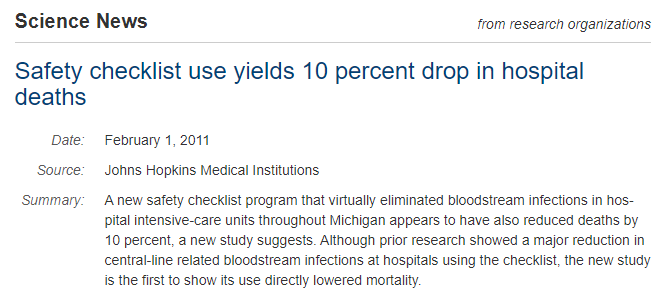
\includegraphics[scale=.6]{graphics/News Clip4.PNG}
\end{frame}

\begin{frame}[fragile]{HIT had Great (Expected) Potential in Healthcare}
\begin{alertblock}{Cost Saving}
\begin{itemize}
    \item A 2005 estimate finds possible cost reduction of hundreds of billions of dollars (\cite{hillestad2005})
\end{itemize}
\end{alertblock}

\begin{alertblock}{Quality Improvement}
\begin{itemize}
    \item Improved efficiency, patient safety improvements, physicians have decision support that could prevent unnecessary complications, etc.
    \item Significant policy push for EHR implementation with these goal in mind: HITECH Act, 2008 provided financial incentive for hospitals to implement EHRs \nocite{hitech}
\end{itemize}
\end{alertblock}

\textcolor{blue}{The percentage of hospitals with basic EHR capability rose from 9$\%$ in 2008 to 84$\%$ in 2015.} (\cite{stats})

\end{frame}

\begin{frame}[fragile]{What does this mean for physicians?}
\begin{itemize}
    \item Initially, this means physicians spend more time entering information into a computer and learning a new software
    \item Loss of autonomy as EHRs have progressed
    \item Physicians have experienced significant burn-out from EHRs
\end{itemize}

\end{frame}

\begin{frame}[noframenumbering]{Physician Burnout}
\begin{center}
    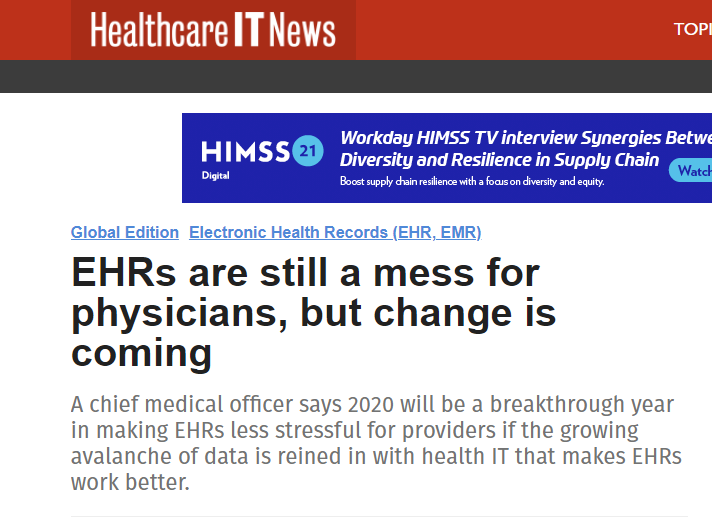
\includegraphics[scale=.4]{graphics/News Clip1.PNG}
\end{center}
\end{frame}

\begin{frame}[noframenumbering]{Physician Burnout}
\begin{center}
    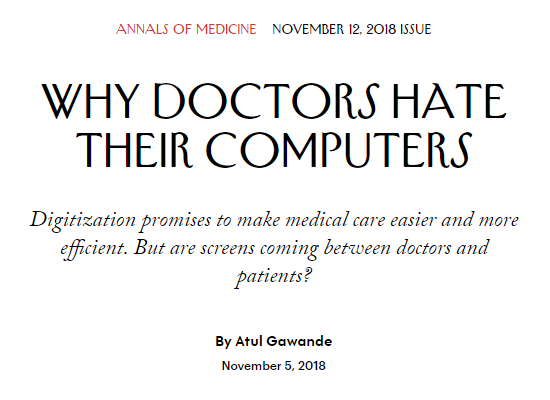
\includegraphics[scale=.5]{graphics/News Clip2.PNG}
\end{center}
\end{frame}

\begin{frame}[noframenumbering]{Physician Burnout}
\begin{center}
    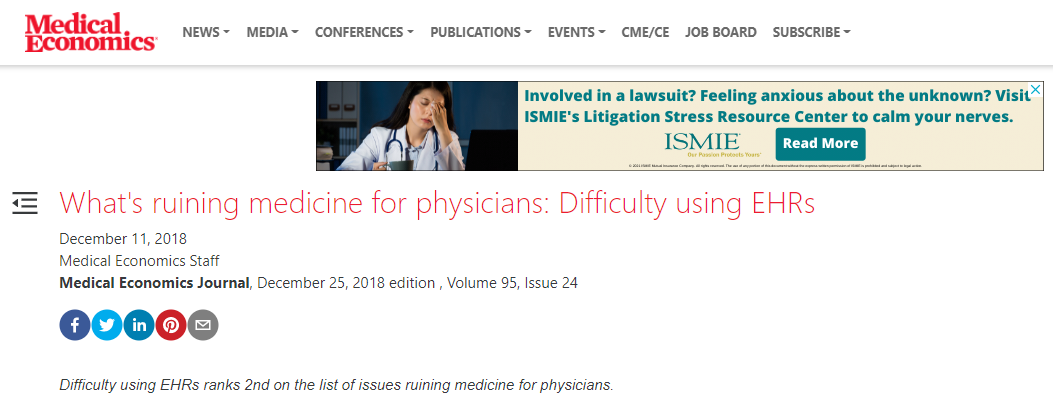
\includegraphics[scale=.45]{graphics/News Clip3.PNG}
\end{center}
\end{frame}

\begin{frame}{This Paper}

Does EHR implementation in hospitals affect labor market decisions of physicians, specifically where, and how much they work?
    
\end{frame}


\section{Contribution}

\begin{frame}{Branches of Literature}
\centering
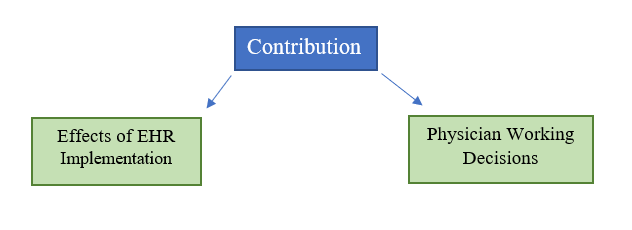
\includegraphics[scale=.5]{graphics/Contribution_litgraphic.PNG}

\end{frame}

\begin{frame}{Physician Labor Literature}
\centering
    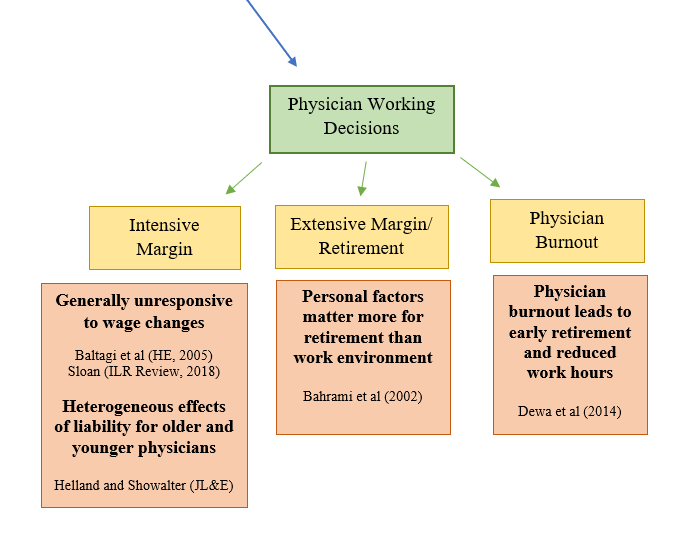
\includegraphics[scale=.45]{graphics/labor_litgraphic.PNG}
\end{frame}

\begin{frame}{EHR Literature}
    \centering
    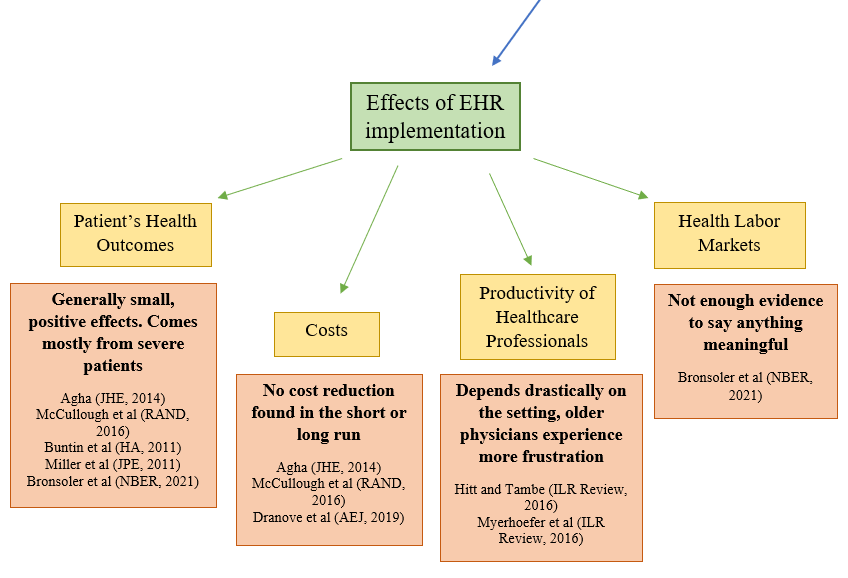
\includegraphics[scale=.45]{graphics/EHR_litgraphic.PNG}
\end{frame}


\section{Data}


\begin{frame}{Physician's Incentives}
\begin{itemize}
    \item Physician decides to work, possibly at a handful of hospitals
    \item Some proportion of these implement a new technology (an EHR)
    \item Two ways to think about the effect:
    \begin{enumerate}
        \item The cost of switching hospitals is higher (attachment to EHR hospital)
        \item The cost of switching hospitals is lower (increased burden at EHR hospital)
    \end{enumerate}
\end{itemize}
\end{frame}


\begin{frame}{Data}
\begin{equation*}
    \textcolor{blue}{p_{iht}}=f(EHR_{ht},EHR_{-h,t},X_i,H_{jt},...)
\end{equation*}

\vspace{3mm}

Measures of physician labor market behavior
\begin{itemize}
    \item Number/percent of shared patients physician $i$ has with hospital $h$: \underline{CMS Shared Patient Data} (2009-2015)
    \begin{itemize}
        \item Main dataset: physician hospital level panel
        \item Physicians and hospitals in this data work closely together, likely the physician works \textit{in} the hospital
    \end{itemize}
    \item Total Part B claims for physician $i$: \underline{Medicare Provider Utilization and Payment Data} (starts in 2012)
\end{itemize}
\end{frame}

\begin{frame}{Data}
\begin{equation*}
    p_{iht}=f(\textcolor{blue}{EHR_{ht},EHR_{-h,t}},X_i,H_{jt},...)
\end{equation*}

\vspace{5mm}

\begin{itemize}
    \item Main variable (binary for whether a hospital uses an EHR) comes from AHA survey
    \item AHA IT Supplement also has information on EHRs that can help with documentation or decision making
    \item (\textit{Considering Later}) Meaningful use data gives information on which hospitals received a subsidy for achieving "meaningful use"
\end{itemize}
\end{frame}

\begin{frame}{Data}
\begin{equation*}
    p_{iht}=f(EHR_{ht},EHR_{-h,t},\textcolor{blue}{X_i},H_{jt},...)
\end{equation*}

\vspace{5mm}

Physician level characteristics
\begin{itemize}
    \item Medical school graduation date, gender: \underline{Physician Compare}
\end{itemize}
\end{frame}

\begin{frame}{Data}
\begin{equation*}
    p_{iht}=f(EHR_{ht},EHR_{-h,t},X_i,\textcolor{blue}{H_{jt}},...)
\end{equation*}

\vspace{5mm}

Hospital Level Characteristics
\begin{itemize}
    \item Number of beds: AHA Survey
    \item Number of days out of the year operating: AHA Survey
\end{itemize}
\end{frame}

\begin{frame}{Summary Statistics}
\centering

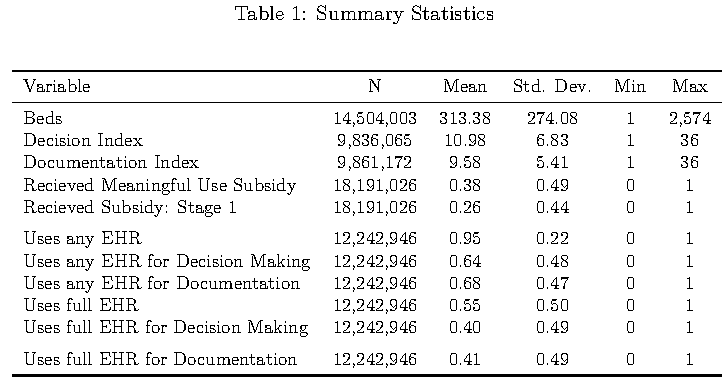
\includegraphics[scale=.8]{Objects/sumstats_pair_table.pdf}

\vspace{3mm}

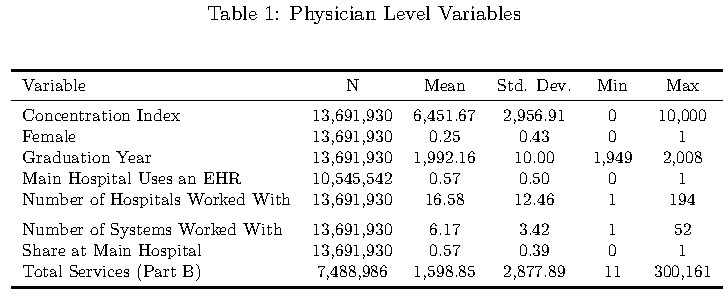
\includegraphics[scale=.8]{Objects/sumstats_physician_table.pdf}

\end{frame}

\begin{frame}{Summary Statistics}
\centering
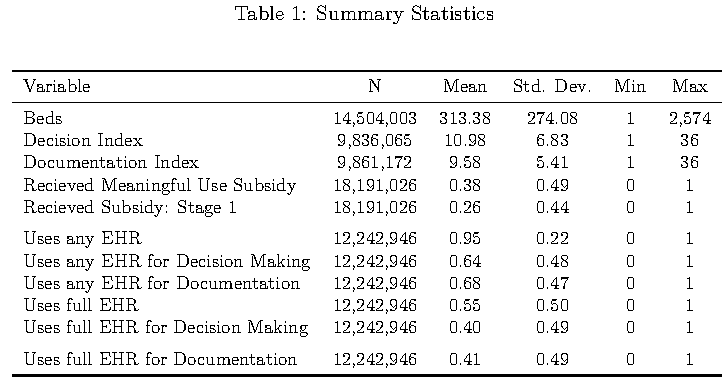
\includegraphics[scale=.8]{Objects/sumstats_hospital_table.pdf}
    
\end{frame}

\begin{frame}{Variation in EHR Adoption}
\centering
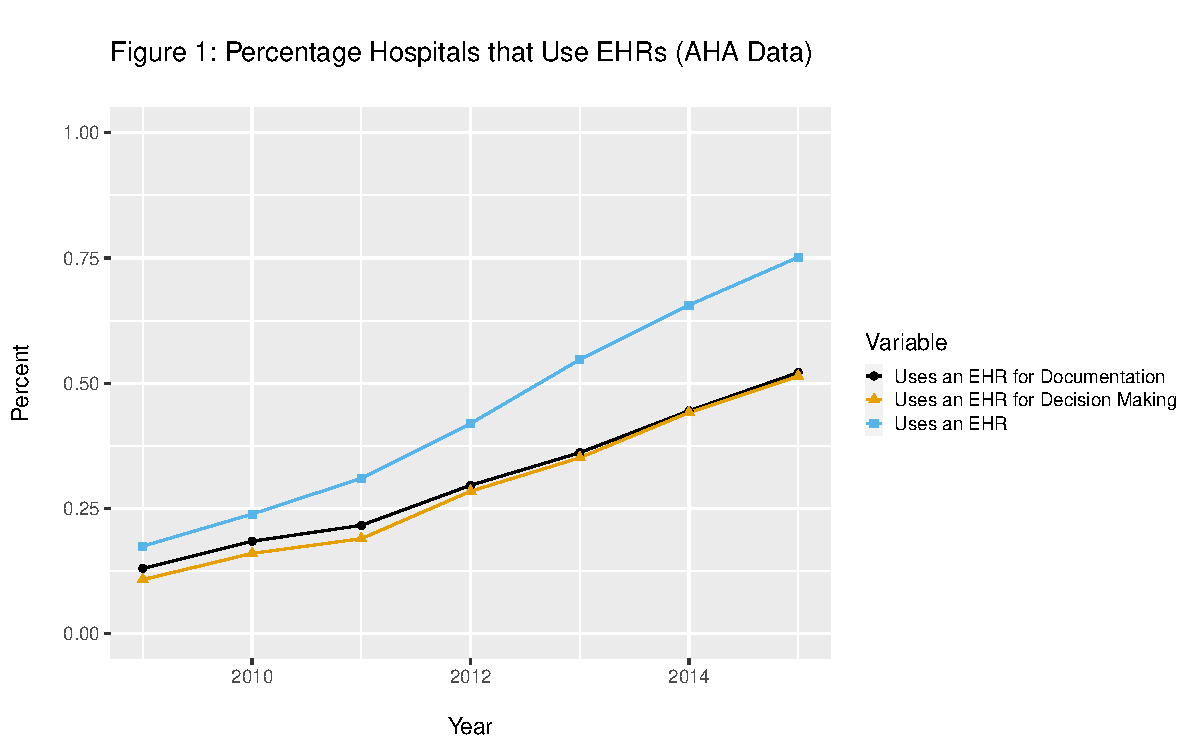
\includegraphics[scale=.53]{Objects/TYP_plot_hospEHR_year.pdf}
\end{frame}

\begin{frame}{Looking at Shares when EHRs are Adopted}
    \centering
    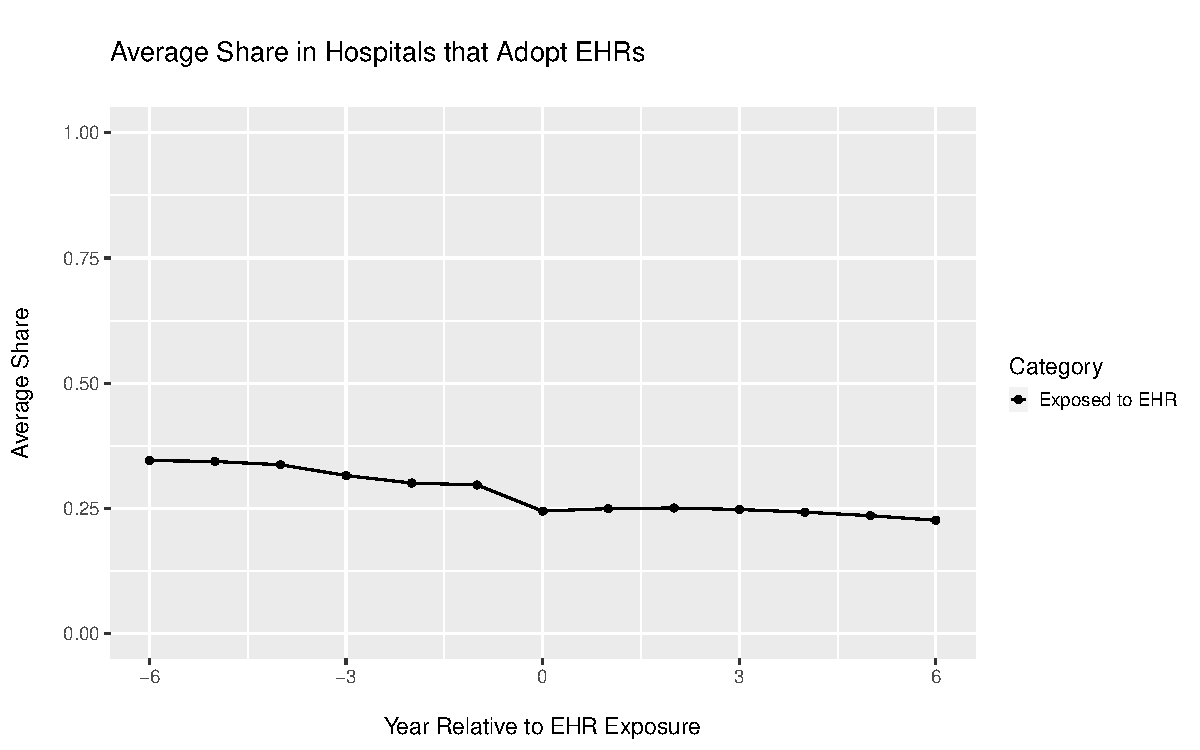
\includegraphics[scale=.5]{Objects/relyear_treatment.pdf}
\end{frame}





\section{Plans}

\begin{frame}{Initial Plan: Difference in Difference}
\begin{itemize}
    \item Interested in two treatment effects
    \begin{enumerate}
        \item The effect of EHR at hospital $h$ on share at hospital $h$
        \item The effect of EHR at hospital $h$ on share at hospital $-h$
    \end{enumerate}
    
    \vspace{2mm}
    
    \item My idea is to estimate these two separately, but there are issues because of spillover effects (hospital $-h$ implements an EHR)
    
    \vspace{2mm}
    
    \item Control group will be physicians who have not yet been exposed to an EHR at \textbf{any} hospital at time $t$
\end{itemize}
\end{frame}

\begin{frame}{Other Ideas}
\begin{itemize}
    \item Aggregate to physician level dataset if there is insufficient data for the control group
    \item Have a continuous measure of EHR use that captures share of exposure to EHRs
    \item IV: bandwidth, state privacy laws
\end{itemize}
\end{frame}

\begin{frame}{Other Points}
\begin{itemize}
    \item Want to dig deeper into how a hospital qualified for meaningful use subsidies
    \item Physician location
    \item Bring in other measures of work from shared patient data
\end{itemize}
    
\end{frame}








\end{document}
